%%%%%%%%%%%%%%%%%%%%%%%%%%%%%%%%%%%%%%%%%%%%%%%%%%%%%%%%%%%%%%%%%%%%%%%%%%%%%%%%%%%%%%%%%%%%%%%%%%%%%%%%%%%%%%%%%%%%%%%%%%%%%%%%%
\chapter{Methodology}
\label{cha:methodology}

%%%%%%%%%%%%%%%%%%%%%%%%%%%%%%%%%%%%%%%%%%%%%%%%%%%%%
\section{Planning}

Planning and task scheduling have been carried using Pivotal Tracker, an online agile project management tool. With this tool, one can estimate his working velocity to make planning decisions based on past performance. It also enable real-time collaboration so that everyone in the team is able to interact with the planning.\\

\begin{figure}[ht]
\center
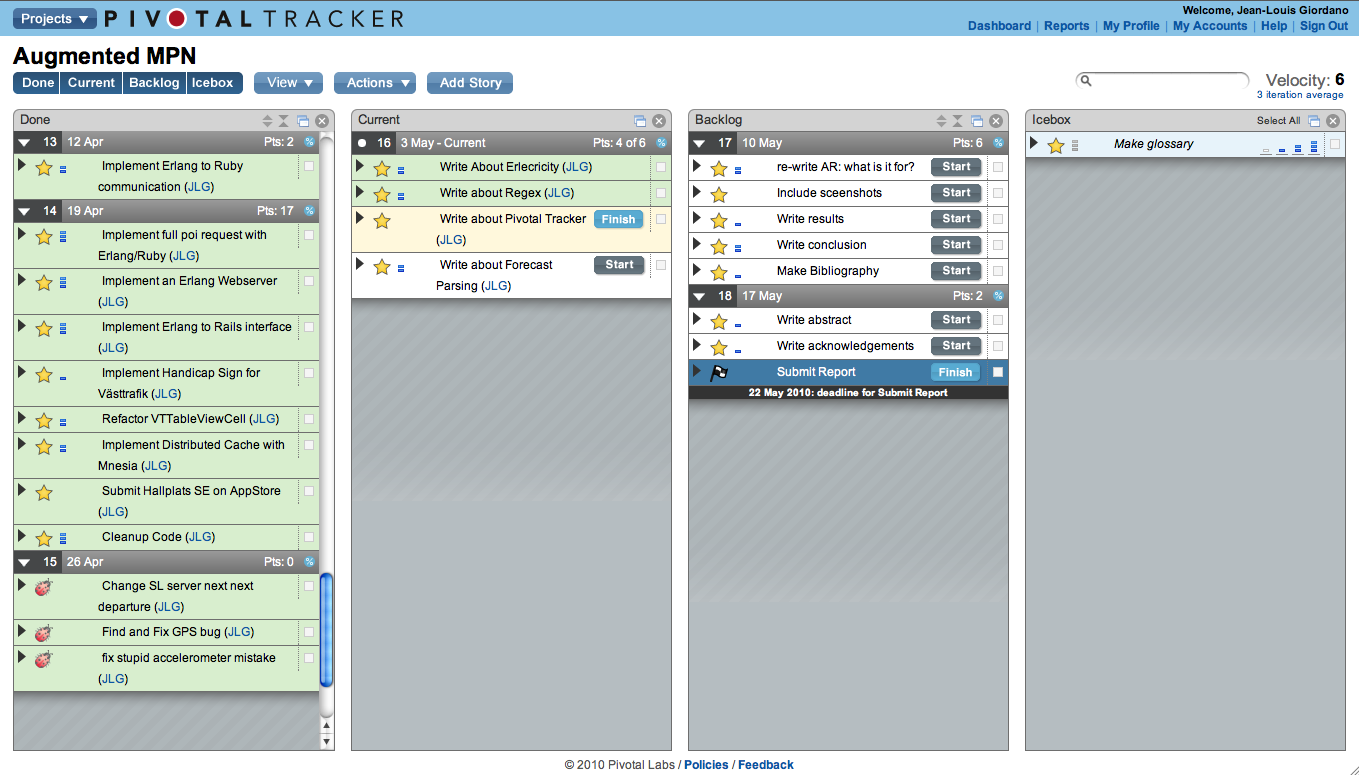
\includegraphics[scale=0.3]{pics/pivotal_tracker}
\caption{Screenshot of the Pivotal Tracker tool}
\label{fig:pivotal_tracker}
\end{figure}

With this tool, a task is represented by a story. A story can be a new feature, a chore, a bugfix or a release date. The last one will appear as a deadline, whereas the others will be represented as a task to be carried out.\\

When creating a new story, one should evaluate the time to be spent on it. This helps the user to estimate his working velocity. A task should be defined such that it would not last longer than half a day.\\

Once the story is added, it is put into an Icebox, which means it is saved but not added to the planning. This can be useful if the story describes an optional feature or idea. Once the user decide that the task should be carried out someday, the story is put in the backlog. Then when the user starts working on the story, it goes to the Current pipe, and when the task is achieved it is kept in the Done stage.\\

This is a really convenient tool, and it has been used from the very beginning of this project both as a reporting and scheduling system.

%%%%%%%%%%%%%%%%%%%%%%%%%%%%%%%%%%%%%%%%%%%%%%%%%%%%%
\section{Version Control}

In order to keep a safe and coherent development process, Git has been used as a version control system. Git is a fast and powerful tool that allows complex revision management, including branching and merging with distributed development.\\

The project is hosted on GitHub, an online Git repository that anyone in the team can access and fork.\\

\begin{figure}[ht]
\center
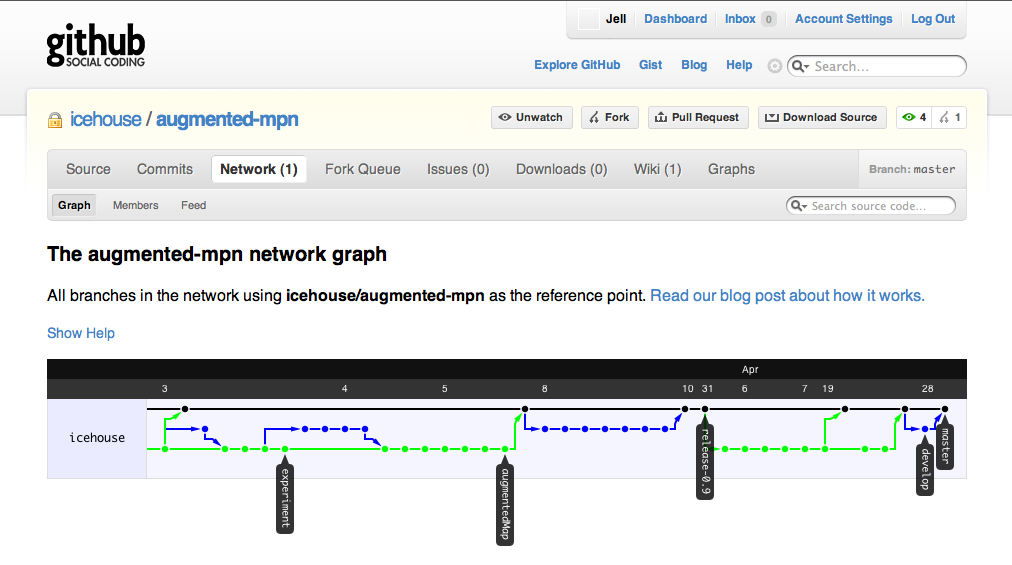
\includegraphics[scale=0.4]{pics/github}
\caption{Screenshot of the GitHub repository}
\label{fig:pivotal_tracker}
\end{figure}

The commits in the Git repository correspond roughly to the stories defined in the Pivotal Tracker (see previous section).